\setcounter{chapter}{1}
%*******************************START INTRODUCTION **********************************
\section{Introduction}\label{sec:intro}
In this chapter we introduce the context of this research, which is about argumentation-based negotiation dialogue games. We also present the motivations behind this work and the research questions. Also, we discuss the objective of this research and our preliminary contributions. Proposal organization is presented in the last section.

\subsection{Context of the research}\label{sec:context}

Autonomous agents and multiagent systems (MAS) provide a technology offering an alternative for the design of intelligent and cooperative
systems. Recently, efforts have been made to develop novel tools, methods, and frameworks to establish the necessary standards for wider
use of MAS as an emerging paradigm ~\cite{Mehdi03}. An increasing interest within this paradigm is on modeling interactions and dialogue systems.
In fact, several dialogue systems have been proposed in the literature for modeling \emph{information seeking} dialogues (e.g.,~\cite{MWParsons03}),
\emph{inquiry} dialogues (e.g.,~\cite{BlackH07,Black09}), \emph{deliberation} dialogues (e.g.,~\cite{Tolchinsky2012}), \emph{persuasion}
dialogues (e.g., ~\cite{Amgoud00}), and \emph{negotiation} dialogues (e.g., ~\cite{KSycara90}), which are our concern in this paper.
Negotiation is a form of interaction in which a group of agents, with conflicting interests, but a desire to cooperate, try to come to a mutually
acceptable agreement on the division of scarce resources~\cite{Rahwan03,Bentahar07}. It is worth noting that in all types of dialogue systems
mentioned above, a dialogue game is a normative model of dialogue, which mainly consists of: i) a set of moves (e.g., challenge, assertion, question, etc.);
ii) one commitment store for each conversant where the advanced moves are stored; iii) a communication language specifying the locution that will be
used by agents during a dialogue for exchanging moves; iv) a protocol specifying the set of rules governing the dialogues; and v) agents' strategies,
which are the different tactics used by agents for selecting their moves at each step in the dialogue~\cite{AmgoudS08}. A dialogue correctly proceeds
as long as the participants conform to the dialogue rules and eventually ends when some termination rules are achieved~\cite{AmgoudS08,Nicolas03,Prakken01}.

In the recent years, argumentation theory has been widely investigated and used to model and analyze dialogue games~\cite{BentaharAIR,BentaharKBS10,Reed06,Mahalakshmi09}.
Argumentation provides a powerful tool to represent, model, and reason about dialogue moves, strategies, and dialogue outcomes. The core idea is the ability
to support moves with justifications and explanations, which play a key role in persuasion and negotiation settings~\cite{GarciaCRS13}. In this paper, we
will focus on the exchanged moves in a dialogue game (i.e., the dialogue itself) and the agents playing these moves when supporting arguments are used.
The main issue we are investigating is the uncertainty index of selecting the right moves during the dialogue, the certainty index that the selected move
will be accepted by the addressee, and the uncertainty index of the whole dialogue. Uncertainty can be thought of as being the inverse of information. Information
about a particular engineering or scientific problem may be incomplete, imprecise, fragmentary, unreliable, vague, contradictory, or even deficient~\cite{RossJA13}.
Uncertainty about values of given variables (e.g., the disease affecting a patient in medical applications) can result from some errors and hence from unreliability
(in the case of sensors) or from different background knowledge (in the case of agents). As a result, it is possible to obtain different uncertain pieces of
information about a given value from different sources~\cite{Jenhani07}. Our aim is to investigate the uncertainty issues that the agent faces when choosing an
argument to play in argumentation-based negotiations. In the literature, many efforts have been deployed to model negotiation. A brief description of those efforts
is given in the following subsection.


A multiagent system is a system where agents (software autonomous entities) are allowed to freely enter and leave the
system, thus making the environment continuously changing. These agents need to communicate with each other, with individual or
collective tasks, with different resources, and different skills. As a result, these agent societies are becoming more and more
similar to the human ones~\cite{Falcone99}.\\
An attractive characteristic of MAS is that agents can act more effectively in groups. Agents are designed to
autonomously collaborate with each other in order to satisfy both their internal goals and the shared external demands
generated by virtue of their participation in agent societies. \\
The languages used by agents to communicate are called Agent Communication Languages (ACLs). The main objective of an
ACL is to model a suitable framework that allows heterogeneous agents to interact and to communicate with meaningful
statements that convey information about their environment or knowledge~\cite{Kone00}. Two main ACLs have been proposed:
the Knowledge Query and Manipulation Language (KQML)~\cite{Finin95}, and the Foundation for Intelligent Physical Agents'
Agent Communication Language (FIPA-ACL)~\cite{Fipa01}.\\
Furthermore, there is an increasing interest on modeling interactions and dialogue systems. Indeed, several
dialogue systems have been proposed in the literature for modeling information seeking dialogues (e.g.~\cite{MWParsons03}),
inquiry dialogues (e.g.,~\cite{BlackH07}), persuasion dialogues (e.g.,~\cite{Amgoud00}) and finally negotiation dialogues
(e.g.,~\cite{KSycara90}).\\
Evaluating multiagent systems and the dialogues taking place between the participants is a very important issue in the recent
developments of multiagent systems. The existing approaches on evaluating these systems are focusing on one aspect at a time, such as
evaluating persuasion dialogues (~\cite{Amgoud00}), and measuring the impact of argumentation (~\cite{Hunter04}). They are more concerned
with proposing dialogue strategies and analyzing dialogues. However, nothing is said about the agents' certainty about their dialogues and
the goodness degree of the agents in the dialogues. In this thesis, we are interested particularly in negotiation dialogue games. In fact,
negotiation is a form of interaction in which a group of agents, with conflicting interests, but a desire to cooperate, try to come to a
mutually acceptable agreement on the division of scarce resources ~\cite{Rahwan03,Bentahar07}. Dialogue games are a set of rules governing the
dialogue. such rules specify the allowed communicative acts agents can perform when participating in  a dialogue. Precisely, we focus in this
work on quantitative negotiation dialogue games such as bargaining. We will focus first on the exchanged moves (i.e. the dialogue itself) in
terms of the certainty index of selecting the right moves during the dialogue, and the certainty index of the whole dialogue. Uncertainty about
values of given variables (e.g. the disease affecting a patient in medical applications) can result from some errors and hence from non-reliability
(in the case of sensors) or from different background knowledge (in the case of agents). As a result, it is possible to obtain different uncertain
pieces of information about a given value from different sources ~\cite{Jenhani07}. The second focus of this thesis is on the agents' strategies in
terms of goodness degree of the agents in the real dialogue (i.e. the dialogue that effectively happened between the participants) and the farness
degree of the agents from the right dialogue (i.e. the best dialogue that can be produced by two agents if they know the knowledge bases of each other).
For example in negotiation setting, the best dialogue is the one in which with a minimum number of moves, two agents can achieve the best agreement for
both of them, if such an agreement exists considering the knowledge bases of these two agents.
%



\subsection{Motivations and research questions}\label{sec:motivation}

Multiagent systems are widely used in everyday life, and to add more value to these systems in the field of software engineering,
they supposed to be measurable. Our motivation is to find a way to measure these systems from different aspects such as measuring
the dialogues, the performance of the participants in the dialogues, and the protocols governing the dialogues, etc. In order to evaluate
dialogues in multiagent systems, we define a new set of measurements from an external agent's point of view. Defining measures for the
participants in the dialogues is another motivation in this thesis. The aim behind developing such measurements is to help engineers and
developers of agent-based systems in evaluating these systems and their performances.\\

\indent When monitoring a dialogue between two or more agents, there are many question that should be answered. In this thesis, we are interested in answering the following questions:

\begin{itemize}
\item How much are agents certain about selecting a move at each dialogue step?
\item How much are agents certain about their dialogues?
\item How good are agents in the real dialogue (i.e. the effective dialogue)?
\item How far are agents from the right dialogue (i.e. the best dialogue given the knowledge bases of the participants)?
\end{itemize}
Answering these questions is undoubtedly complex. Therefore, we do not expect a comprehensive answer to all these questions.



\subsection{Research objectives and contributions}\label{sec:contribution}

The main objective of this thesis is to develop a new set of measurements for negotiation dialogue games to help in evaluating and
comparing different negotiation dialogues with different participants for the same topic. The importance of introducing measures for
negotiation dialogue games at each step of the dialogue such as measuring how much the agent is certain about its move is to help in developing intelligent multiagent systems (MAS) and to help evaluating different agents provided by different developers.\\
\indent Our research aims to ensure that the agents' certainty about their dialogue is fairly represented at each step during
the dialogue by making sure that the agent's certainty about selecting the right move is kept in mind and considered as a property
of multiagent systems.\\
\indent The main contribution of this thesis is the proposition of a new set of measures for dialogue games from an external agent's point of view.
In particular, we introduce two sets of measurements. In the first set  we use Shannon entropy to measure the certainty index of the dialogue.
This involves i) using Shannon entropy to measure the agent's certainty about each move during the dialogue; and ii) using
Shannon entropy to measure the certainty of the agents about the whole dialogue with two different ways. The first way is
by taking the average of the certainty index of all moves, and the second way is by determining all possible dialogues and
applying the general formula of Shannon entropy. In the second set, we are measuring how good are agents in the real dialogue
\emph{(Goodness Degree )}, and measuring how far are agents from the right dialogue \emph{(Farness Degree)}~\cite{Marey09}.



As mentioned earlier, there exist several proposals on the argumentation-based negotiation. Most of them are concerned with proposing protocols to show how agents can
interact with each other, and how arguments and offers can be generated, evaluated and exchanged during the negotiation process. However, none of them has investigated
the agents' uncertainty about the exchanged arguments and how such an uncertainty could be measured at each dialogue step to assist the agents make a better decision. The
uncertainty is generally defined as ``that which is not precisely known''. This definition permits the identification of different kinds of uncertainty arising from different
sources and activities, most of which go unnoticed in analysis. To the best of our knowledge, this work is the first of it's kind in dealing with the agent's uncertainty
while making a decision at each dialogue step in order to achieve an agreement. In this paper, we define a new set of uncertainty measures for dialogue games from an
external agent's point of view. In particular, we distinguish two types of uncertainty: \textbf{Type I} and \textbf{Type II}.

Type I is about the uncertainty of playing the right move (i.e., advancing the right argument) at each dialogue step. For this type, we use Shannon entropy to measure: i) the
uncertainty index of the agent that he is selecting the right move at each step during the dialogue; and ii) the uncertainty index of both agents participating in the dialogue
about the whole dialogue. The latter measurement will be conducted in two different ways. The first way is by taking the average of the uncertainty index of all moves,
and the second is by determining all possible dialogues based on the union of the agents' knowledge bases and applying the general formula of Shannon entropy.

Type II is about the uncertainty of the agent that the selected move (argument) will be accepted by the addressee (from now on we will call this second type of uncertainty
by \emph{uncertainty degree}). In this context, we introduce a new classification of arguments based on their certainty index. These measures are of great importance since
they can be used as guidelines for a protocol in order to generate the best dialogue between autonomous intelligent agents.

Figure \ref{fig1.0} summarizes the whole proposed approach where the certainty index ($CI$) and weighted certainty index ($W\_CI$) of the moves and the whole dialogue are
measured for Type I. For Type II, different cases are considered depending on how many arguments are in use.

\begin{figure}[t]
                \begin{center}
                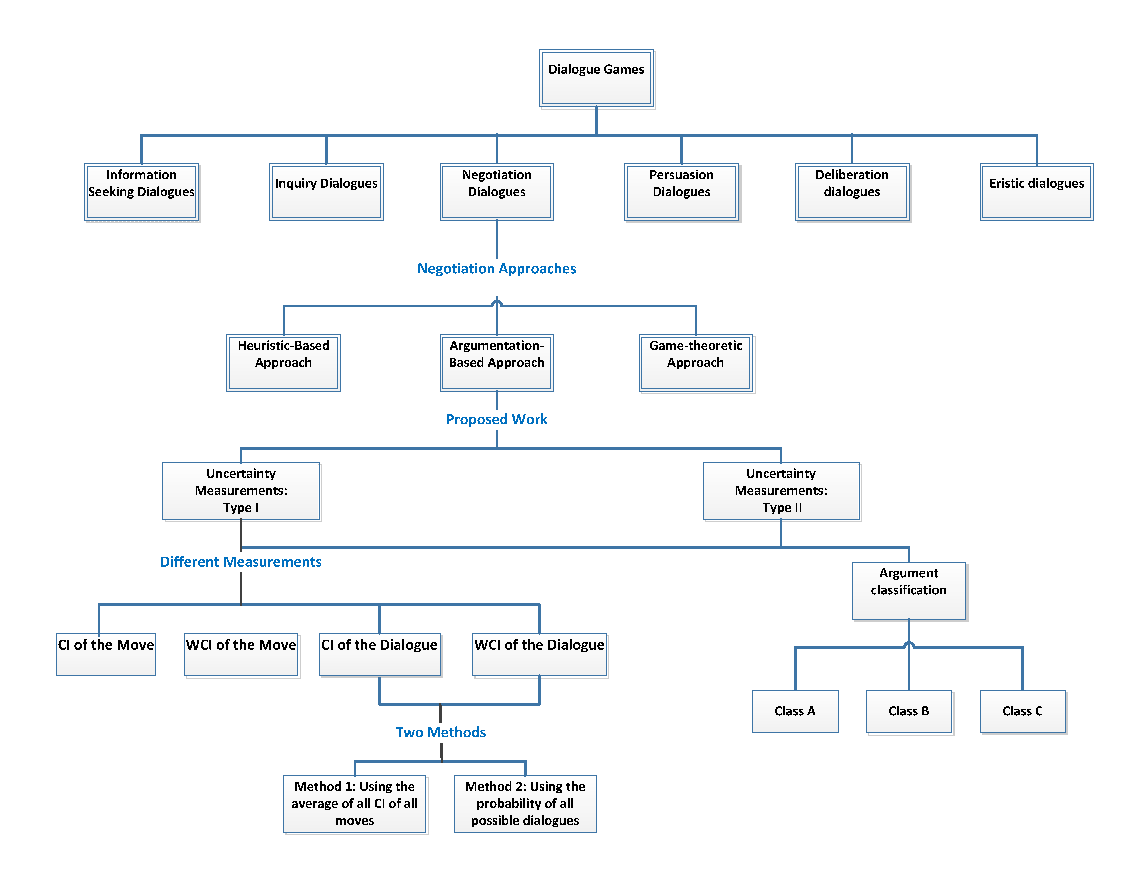
\includegraphics[width=15cm, height=11cm]{Figures/Approach1.eps}
                \end{center}
                \caption{General overview of the approach}\label{fig1.0}
                \label{Stack}
                \end{figure}


\subsection{Research outline}\label{sec:outline}
The rest of the paper is organized as follows: In Section~\ref{sec:Argumentation}, we present a  brief theoretical background on the argumentation system
and agent's theory, strategic reasoning, tactic reasoning and risk of failure notions are also discussed in this section. In Section~\ref{sec:uncertainty},
we present the agent's uncertainty measures using Shannon entropy, which include type I (measuring the uncertainty of the agent about selecting the right move)
and type II (measuring the uncertainty degree that the selected move will be accepted). Argument classification is also presented in this section. Related work
is discussed in Section~\ref{sec:related}. Finally, conclusion and future work are presented in Section~\ref{sec:conclusion}.






%****************************************** END INTRODUCTION****************************************
